\documentclass[tikz,border=15pt]{standalone}
\usepackage{amsmath,amssymb}

\begin{document}
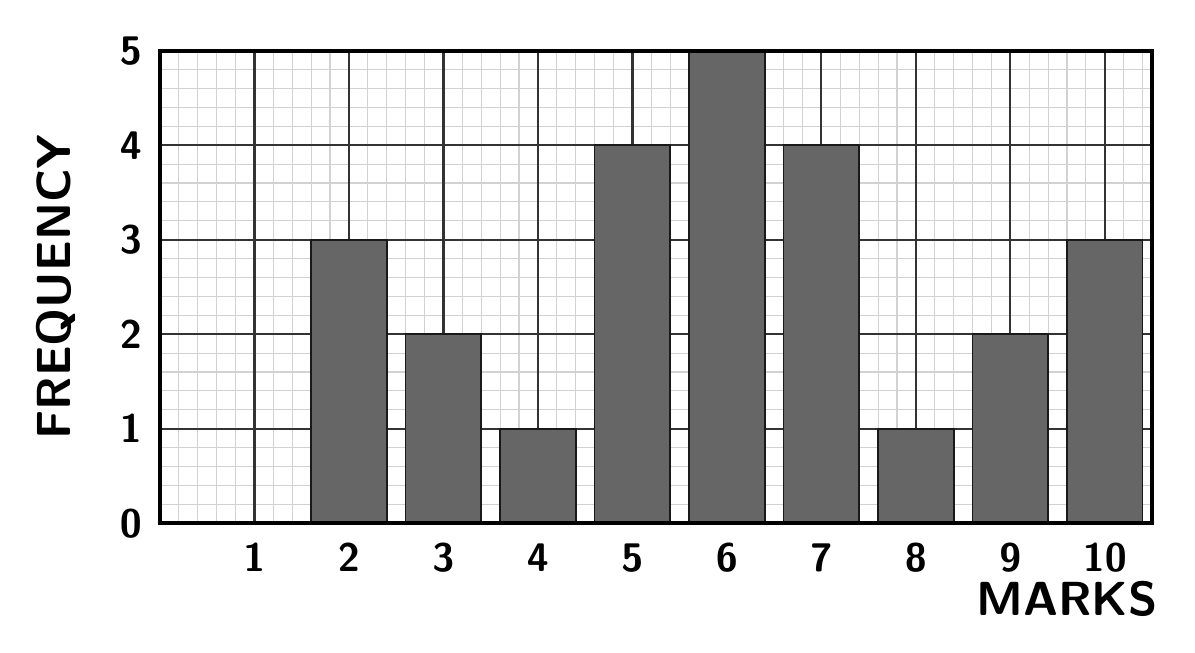
\begin{tikzpicture}[scale=1.2]
    % Fine graph paper grid (subdivisions of 0.2)
    \draw[step=0.2, gray!35, line width=0.4pt] (0, 0) grid (10.5, 5.0);
    
    % Major grid lines (every 1.0 unit)
    \draw[step=1.0, black!80, line width=0.8pt] (0, 0) grid (10.5, 5.0);
    
    % Solid bars (width 0.8 centered on mark integer)
    % (Mark, Freq): 2->3, 3->2, 4->1, 5->4, 6->5, 7->4, 8->1, 9->2, 10->3
    \foreach \m/\f in {2/3, 3/2, 4/1, 5/4, 6/5, 7/4, 8/1, 9/2, 10/3} {
        \fill[black!60, draw=black!90, line width=0.6pt] ({\m - 0.4}, 0) rectangle ({\m + 0.4}, \f);
    }
    
    % Outer boundary frame
    \draw[line width=1.4pt] (0, 0) rectangle (10.5, 5.0);
    
    % Y-axis labels (0 to 5)
    \foreach \y in {0, 1, 2, 3, 4, 5} {
        \node[left=3pt, font=\Large\sffamily\bfseries] at (0, \y) {\y};
    }
    
    % X-axis labels (1 to 10)
    \foreach \x in {1, 2, 3, 4, 5, 6, 7, 8, 9, 10} {
        \node[below=4pt, font=\Large\sffamily\bfseries] at (\x, 0) {\x};
    }
    
    % Axis Titles
    \node[rotate=90, font=\LARGE\sffamily\bfseries] at (-1.1, 2.5) {FREQUENCY};
    \node[below=18pt, font=\LARGE\sffamily\bfseries] at (9.6, 0) {MARKS};
    
\end{tikzpicture}
\end{document}
